%% Преамбула TeX-файла

% 1. Стиль и язык
\documentclass[utf8x]{G7-32} % Стиль (по умолчанию будет 14pt)
\usepackage[T2A]{fontenc}
\usepackage[russian]{babel}
% Остальные стандартные настройки убраны в preamble.inc.tex.
\sloppy

% Настройки стиля ГОСТ 7-32
% Для начала определяем, хотим мы или нет, чтобы рисунки и таблицы нумеровались в пределах раздела, или нам нужна сквозная нумерация.
\EqInChapter % формулы будут нумероваться в пределах раздела
\TableInChapter % таблицы будут нумероваться в пределах раздела
\PicInChapter % рисунки будут нумероваться в пределах раздела

% Добавляем гипертекстовое оглавление в PDF
\usepackage[
bookmarks=true, colorlinks=true, unicode=true,
urlcolor=black,linkcolor=black, anchorcolor=black,
citecolor=black, menucolor=black, filecolor=black,
]{hyperref}

% Изменение начертания шрифта --- после чего выглядит таймсоподобно.
% apt-get install scalable-cyrfonts-tex

\IfFileExists{cyrtimes.sty}
    {
        \usepackage{cyrtimespatched}
    }
    {
        % А если Times нету, то будет CM...
    }

\usepackage{graphicx}   % Пакет для включения рисунков

% С такими оно полями оно работает по-умолчанию:
% \RequirePackage[left=20mm,right=10mm,top=20mm,bottom=20mm,headsep=0pt]{geometry}
% Если вас тошнит от поля в 10мм --- увеличивайте до 20-ти, ну и про переплёт не забывайте:
\geometry{right=20mm}
\geometry{left=30mm}


% Пакет Tikz
\usepackage{tikz}
\usetikzlibrary{arrows,positioning,shadows}

% Произвольная нумерация списков.
\usepackage{enumerate}

% ячейки в несколько строчек
\usepackage{multirow}

% itemize внутри tabular
\usepackage{paralist,array}


% Полезные макросы листингов.
% Любимые команды
\newcommand{\Code}[1]{\textbf{#1}}

%% Перенос знаков в формулах (по Львовскому)
\newcommand*{\hm}[1]{#1\nobreak\discretionary{}
{\hbox{$\mathsurround=0pt #1$}}{}}


\begin{document}
\frontmatter % выключает нумерацию ВСЕГО; здесь начинаются ненумерованные главы: реферат, введение, глоссарий, сокращения и прочее.

% Команды \breakingbeforechapters и \nonbreakingbeforechapters
% управляют разрывом страницы перед главами.
% По-умолчанию страница разрывается.

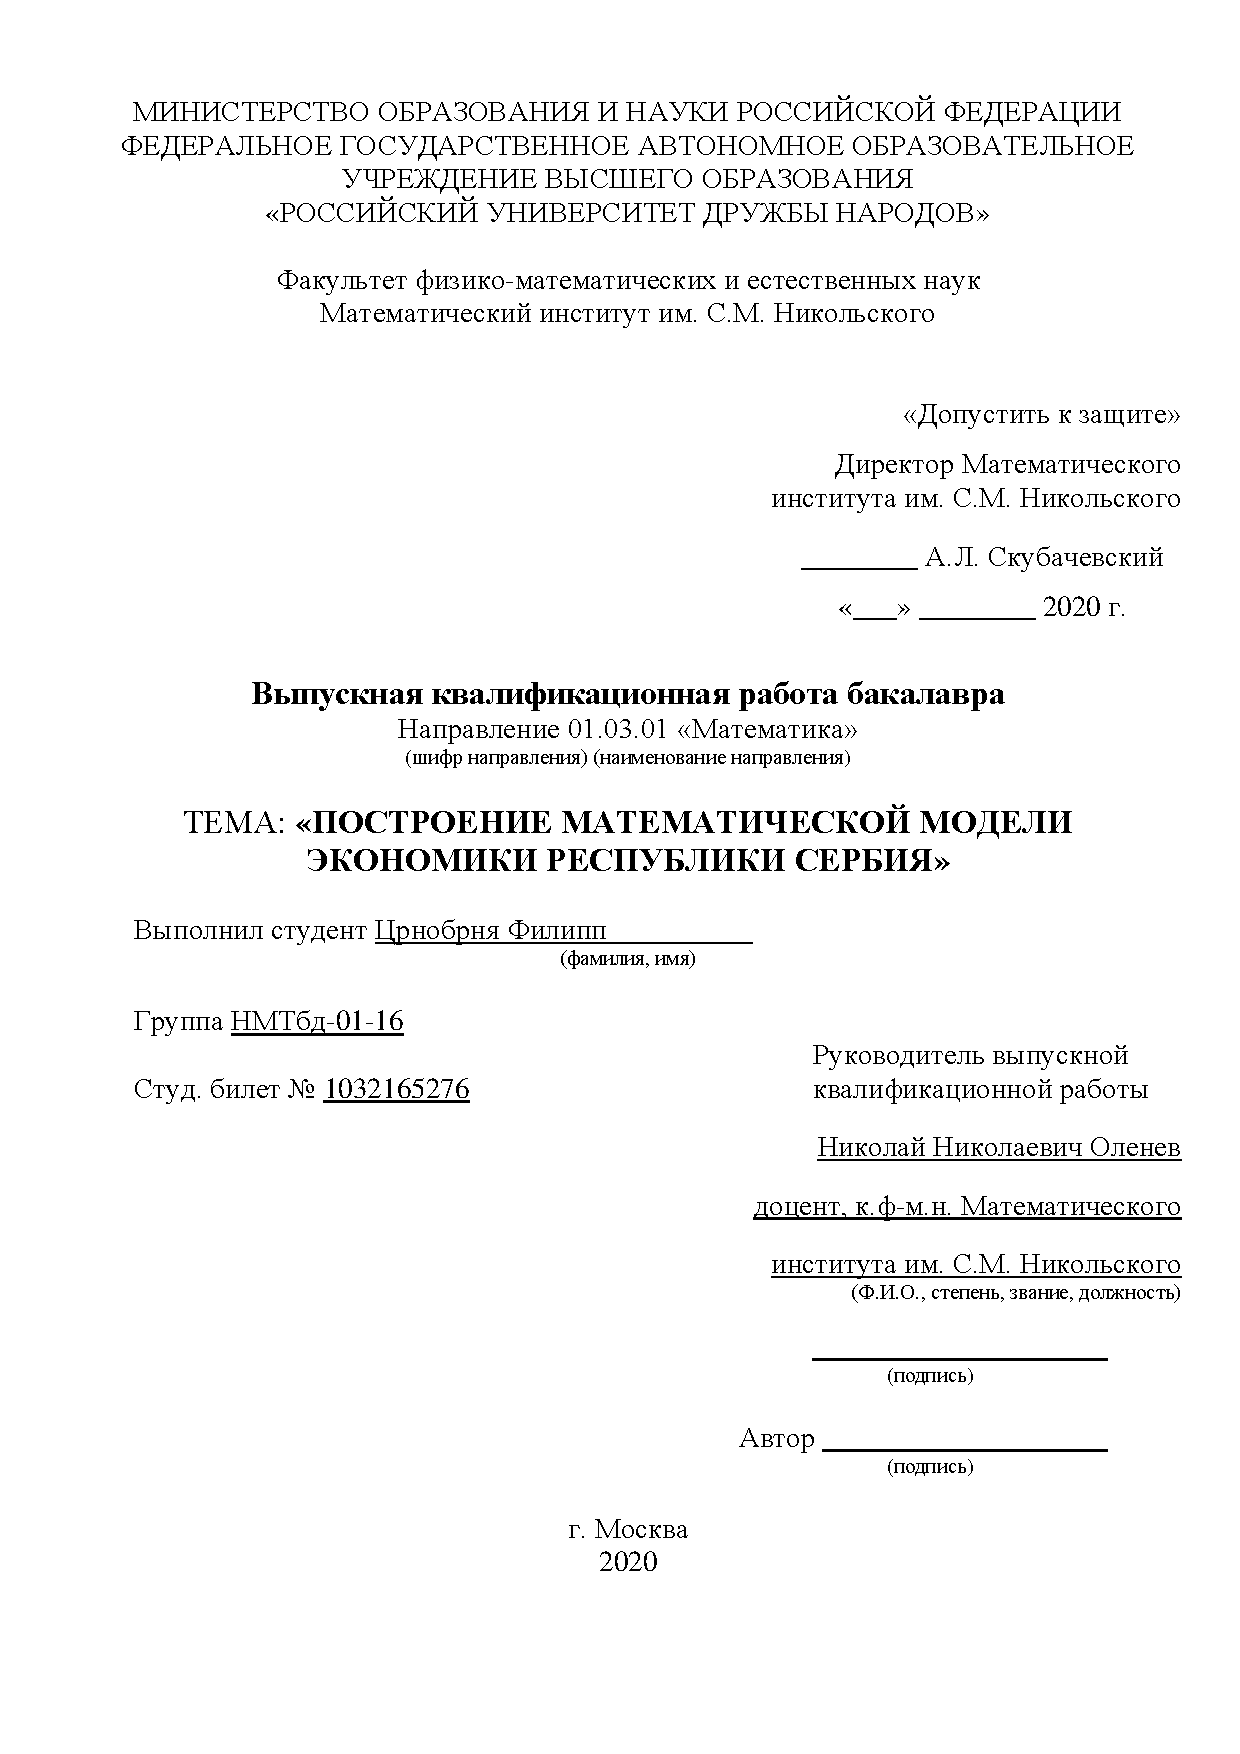
\includepdf{inc/title.pdf}
% \nobreakingbeforechapters
\breakingbeforechapters


\tableofcontents

\Abbreviations %% Список обозначений и сокращений в тексте
\begin{description}
\item[ООН] Организация Объединённых Наций.
\item[МВФ] Международный Валютный Фонд.
\item[ВВП] Валовой внутренний продукт.
\item[ИТ] Информационные технологии.
\item[RSD] Сербский динар.
\item[USD] доллар США.
\item[НАТО] Организация Североатлантического договора, Североатлантический Альянс (англ. North Atlantic Treaty Organization).
\item[ПИИ] Прямые иностранные инвестиции.
\item[США] Соединенные Штаты Америки.
\end{description}

%%% Local Variables:
%%% mode: latex
%%% TeX-master: "rpz"
%%% End:

\Introduction

Республика Сербия --- индустриально-аграрная страна, расположенная на юго-востоке Европы (Западные Балканы).
Республика является связывающим звеном между Центральной Европой и Ближним Востоком.
Через страну проходят торговые и транспортные пути.
Республика Сербия имеет запасы полезных ископаемых --- руды цветных металлов, каменный уголь и т.~д.
Через страну протекают крупные реки (Дунай, Сава, Дрина и т.~д.).

На рубеже 1980 -- 1990 годов страна (на тот момент Югославия) была экономически развитой.
Однако политические события 90-х (уничтожение промышленности в ходе многочисленных воздушных атак НАТО, война, санкции ООН, утрата всех связей внутри бывшей Югославии и т.~д.) оказали негативное влияние на экономическое и политическое положение страны.

За последние годы в Сербии начался стремительный экономический рост, возобновились иностранная финансовая помощь и инвестиции.
За 10-летний период по данным МВФ сербская экономика выросла почти на 20 процентов.

Сельское хозяйство, промышленность и сектор услуг являются основными источниками доходов Сербии.
Они внесли большой вклад в динамику роста ВВП.
Основная отрасль сельского хозяйства --- растениеводство.
В обрабатывающей промышленности ведущее место занимают машиностроение и металлообработка.
Также уверенными темпами развиваются ИТ и туризм.
Например, экспорт ИТ сектора в 2019 году был выше, чем экспорт доминирующего сельского хозяйства.
Примечательно, что в 2019 году Балканская республика наряду с Ирландией показала самый высокий экономический рост среди всех остальных государств Европы.
В 2020 году Сербия также может показать опережающию темпы роста экономики в Европе.

\textbf{Актуальность выбранной темы выпускной квалификационной работы } обусловлена тем, что экономика Сербии в настоящий момент находится на этапе активного развития.
Математические модели способны описать текущую экономическую ситуацию в стране и спрогнозировать как и положительные, так и отрицательные сюжеты развития государства.

Экономика государства очень сильно зависит от политической ситуации, она настолько динамична, что построив математическую модель вчера, сегодня она уже может оказаться не актуальной. В связи с вспышкой пандемии COVID-19\footnote{COVID-19 (аббревиатура от англ. COronaVIrus Disease 2019), коронавирусная инфекция 2019-nCoV --- потенциально тяжёлая острая респираторная инфекция, вызываемая коронавирусом \cite{wiki:Coronavirus_disease_2019}.}, многие страны уже оказались в неприятной экономической ситуации.
Это еще одна причина выбора темы.
Кроме того, построение математических моделей экономики государства на примере Сербии поможет разобраться как в особенностях государства, так и в математических инструментах.

\textbf{Объект исследования} --- математические модели экономического роста.

\textbf{Предмет исследования} --- математическая модель экономики, построенная на примере Республики Сербия.

\textbf{Цель данной работы} --- смоделировать динамику экономики Республики Сербия в зависимости от поведения внутренних и внешних переменных и сделать выводы.

Для реализации поставленной цели необходимо решить следующие задачи:
\begin{enumerate}
	\item Изучить теорию построения математических моделей экономики.
	\item Построить модель на примере макроэкономических данных Республики Сербия.
	\item Сделать выводы.
\end{enumerate}

Выпускная квалификационная работа состоит из содержания, перечня сокращений, введения, пяти глав, заключения, списка используемых источников и приложения.

В первой главе определяются основные термины, описываются этапы построения математических моделей, приводятся различные типы математических моделей.

Во второй главе описывается теоретическая состовляющая математической модели экономического роста Солоу.

В третьей главе рассчитываются основные макроэкономические переменные экономики Республики Сербия.

В четвертой главе проводится анализ, вычисления и построение математической модели экономики Республики Сербия, разбираются полученные результаты.

В пятой главе исследуются главные сферы экономической деятельности Сербии, оцениваются прогнозы авторитетных рейтинговых агенств (МВФ, Всемирный банк и т.~д.).


\mainmatter % это включает нумерацию глав и секций в документе ниже
\chapter{Понятие математической модели}
\label{cha:definition}

\section{Основные понятия}

Объект --- система состоящая из множества элементов.
Это может быть ракета, рынок ценных бумаг или популяции животных.
В нашем случае это государство.

Модель несет в себе отражение связей между элементами.
Математическая модель --- это математическое представление реальности.
Экономической моделью можно считать набор уравнений, основанных на определенных предположениях и приближено описывающих экономику в целом или отдельно ее отрасль.

Моделирование --- процесс расчета поведения системы на основе граничных условий и заданных связей между элементами системы.

Алгоритм --- логика расчета поведения системы.
Логика может быть основана на разных математических подходах.

\section{Этапы построения математической модели}

Построение математических моделей в экономике является методом для решения задач оптимального упраления.
Экономико-математическая модель отображает некоторые процессы, которые смоделированы с помощью математических теорем и уравнений.

Построение математических моделей состоит из нескольких этапов:
\begin{itemize}
	\item \textbf{Идентификация.}
	Определение основных параметров объекта.
	\item \textbf{Оценка параметров модели.}
	Выбор переменных модели на основе выбранных параметров.
	\item \textbf{Спецификация модели.}
	Определение связей между параметрами.
	Построение уравнений.
	\item \textbf{Моделирование.}
	Проведение моделирования на основе заданных начальных условий.
	\item \textbf{Анализ полученных результатов.}
\end{itemize}

\section{Классификация математических моделей}

Формальная классификация моделей основывается на классификации используемых математических средств.
Например:
\begin{itemize}
	\item \textbf{Линейные и нелинейные модели.}
	Модели, в которых связь между зависимой и независимой переменными могут быть линейными или нелинейными (например, линейная регрессия).
	\item \textbf{Дискретные и непрерывные модели.}
	В дискретных моделях изменение параметров связано только с отдельными моментами времени.
	В непрерывных моделях параметры изменяются во времени плавно.
	\item \textbf{Стохастические модели.}
	Стохастические модели предназначены для прогнозирования экономических явлений в условиях неопределенности исходных данных и реализуются методами математической статистики.
	\item \textbf{Оптимизационные модели.}
	Оптимизационная модель позволяет из нескольких альтернативных вариантов выбрать наилучший вариант по любому признаку.
\end{itemize}
Естественно, что существуют и другие модели, в том числе и смешанные.

Вся теория построения математических моделей основывается на предположениях, которые не всегда являются правдивыми.
Эти предположения помогает существенно упростить описание какого-либо процесса.
Грамотное построение моделей заключается в создании предположений таким образом, чтобы окончательные результаты оказались наиболее независимыми.
В современной экономической науке модель является математическим описанием отдельных экономических явлений.
Лучшие модели обычно очень просты, но позволяют глубоко описать устройство мира.

\chapter{Модель Солоу}
\label{cha:solow_models}

В этой главе будет описана модель экономического роста, предложенная Робертом Солоу\footnote{Роберт Мертон Солоу (англ. Robert Merton Solow; род. 23 августа 1924, Бруклин, Нью-Йорк) --- американский экономист, лауреат Нобелевской премии 1987 года «за фундаментальные исследования в области теории экономического роста»\cite{wiki_solow}.}.
Эта модель способна объяснить, почему одни страны процветают, а другие становятся все беднее.

Предположим, что мир состоит из стран, в которых потребляется только один товар (выпуск).
Из этого следует, что в мире не существует международной торговли.
В модели рассматривается закрытая экономика\footnote{Отсутствие международных сделок.}.
Вторая предпосылка этой модели заключаетя в том, что технологии не зависят от производителей.

\section{Базовая модель Солоу}

Модель основывается на двух функциях:
\begin{itemize}
	\item Производственная функция.
	\item Уравнение, описывающее процесс накопления капитала.
\end{itemize}
Производственная функция описывает использование ресурсов для производства выпуска\footnote{Выпуск состоит не только из физических единиц.}.
Разделим все ресурсы на:
\begin{itemize}
	\item Труд.
	\item Капитал.
\end{itemize}
Введем специальные обозначения.
\begin{table}[ht]
	\centering
	\caption{Специальные обозначения для производственной функции}
	\begin{tabular}{|r|l|}
		\hline
		Описание & Обозначение \\ \hline
		Капитал  &      $K$    \\
		Труд     &      $L$    \\
		Выпуск   &      $Y$    \\ \hline
		\end{tabular}%
	\label{tab:prod_func}
\end{table}
Предполагается, что производственная функция является функцией Кобба-Дугласа:
\begin{equation}
	Y = F(K, L) = K^{\alpha}L^{1-\alpha}\text{,}
\label{F:Cob_Duglas}
\end{equation}
где $\alpha$ --- некий коэффициент в интервале от 0 до 1.

Работадатель платят рабочим заработную плату $w$ за каждую единицу труда и платят $r$ за аренду единицы капитала.
Пусть цена единицы выпуска равна 1, тогда получим задачу, которая максимизирует прибыть фирме:
\begin{equation}
	\max\limits_{K, L} F(K,L) - rK - wL\text{.}
\end{equation}

Фирмы будут нанимать работников, пока продукт труда не станет равным заработной плате.
\begin{equation*}
	w = \cfrac{\partial F}{\partial L} = \left(1-\alpha\right)\cfrac{Y}{L}\text{.}
\end{equation*}
И арендовать капитал, пока продукт капитала не станет равным его арендной цене.
\begin{equation*}
	r = \cfrac{\partial F}{\partial K} = \alpha\cfrac{Y}{K}\text{.}
\end{equation*}

$wL + rK = Y$, следовательно платежи за реурсы соответствуют объему произведенного выпуска, а значит отсутствует прибыль.

Перепишем производственную функцию \ref{F:Cob_Duglas} как функцию выпуска в расчете на одного работника, зависящую от капитала на одного работника.
\begin{align*}
y = \cfrac{Y}{L}\text{,}\\
k = \cfrac{K}{L}\text{.}
\end{align*}
Получим производственную функцию в новом виде:
\begin{equation}
	y = k^{\alpha}\text{.}
\end{equation}

Второе ключевое уравнение модели Солоу описывает процесс накопления капитала:
\begin{equation}
\dot{K} = sY-\delta K \text{.}
\label{F:capital_solow}
\end{equation}

Величина в левой части уравнения \ref{F:capital_solow} представляет собой аналог дискретной величины $K_{i-1} - K_{i}$.
Это изменение запаса капитала за период.
Второй член выражения обозначает совокупные инвестиции.
Экономика закрытая, поэтому сбережения равны инвестициям.
Третий член уравнения отображает амортизацию капитала в процессе производства.
Часто предполагается, что $\delta = 0,05$.
Это означает, что 5 процентов машин и сооружений выбывает из процесса производвства каждый период.

Рассмотрим темп прироста численности труда $\cfrac{\dot{K}}{K}$.
Предположим, что уровень участия в рабочей силе постоянен, а темп припоста численности населения обозначается с помощью параметра $n$.
Таким образом, темп прироста численности  занятых равен $n$.
Если $n = 0,01$, это обозначает, что тем прироста численности занятых увеличивается на 1 процент.

Для того, чтобы показать каким образом во времени меняется выпуск в расчете на одного работника, возьмем логарифм, а затем производные по времени для уравнения \ref{F:capital_solow}.
\begin{equation*}
\cfrac{\dot{k}}{k} = \cfrac{sY}{K} - n - \delta = \cfrac{sy}{k} - n - \delta\text{.}
\end{equation*}
Это уравнение позволяет получить уравнение, показывающее изменение во времени капиталовооруженности труда:
\begin{equation*}
\dot{k}=sy-(n + \delta)k\text{.}
\end{equation*}

\chapter{Идентификация параметров}
\label{cha:ident_params}

Для построения математической модели воспользуемся макроэкономическими показатели статистического агенства ООН \cite{unstat}.
Так как модели у нас рассматривают закрытую экономику, то нас интересуют данные в национальной валюте Республики Сербия (RSD).

Существует два вида цен:
\begin{itemize}
	\item \textbf{Текущие.}
	Цены на какую-либо конкретную дату, например на 1 апреля, либо средние за год цены.
	\item \textbf{Постоянные.}
	Цены определенного периода, принимаемые за основу расчета макроэкономических показателей.
	Эти цены не учитывают уровень инфляции.
	На момент написания работы этот период --- 2015 год.
\end{itemize}
Если периоды текущих и постоянных цен совпадают, то и цены тоже соответственно совпадают.

Введем специальные обозначения, которые представлены в таблице \ref{tab:desig_of_params}.
\begin{table}[ht]
	\centering
	\caption{Специальные обозначения для параметров.}
	\begin{tabular}{|r|l|}
	\hline
	\multicolumn{1}{|r|}{Параметр} & \multicolumn{1}{l|}{Описание} \\ \hline
	$t$                          & Год - 2010                                            \\
	$Y$                          & ВВП                                                   \\
	$I$                          & размер инвестиций                                     \\
	$C$                          & общие расходы на потребление                          \\
	$L$                          & количество трудящегося населения\footnotemark         \\ \hline
	\end{tabular}
	\label{tab:desig_of_params}
\end{table}
\footnotetext{Трудящееся население включает людей в возрасте 15 лет и старше, которые способны производить товары и услуги в течение определенного периода.Значение включает людей, которые в настоящее время работают, и людей, которые являются безработными, но ищут работу, а также впервые ищущих работу. Однако не все, кто работают, включены. Неоплачиваемые работники, семейные работники и студенты часто не учитываются, а некоторые страны не учитывают военнослужащих. Численность рабочей силы имеет тенденцию меняться в течение года, когда сезонные работники приходят и уходят.}

Таблицы найденных статистических данных для Республики Сербия представлены в приложении \ref{cha:first_app}.
Все найденные показатели представлены в текущих и постоянных ценах.
Все данные представлены с 1993 года, так как это был переломный момент в истории страны.

Первым делом посчитаем индексы цен, определим поведение цен в среднем.
Индекс цен представляет собой соотношение макроэкономических показателей данного периода в текущих и постоянных ценах.
Для этого воспользуемся формулой:
\begin{equation*}
	P(X(t)) = \cfrac{X(t)}{X_{const}(t)}
\end{equation*}
где $X(t)$ --- это макроэкономический показатель за определенный период в текущих ценах.
А $X_{const}(t)$ соответственно в постоянных ценах.

На графике ниже видна динамика поведения цен.
\begin{center}
	\captionof{figure}{Индекс цен (RSD)}
	\begin{tikzpicture}
		\begin{axis}[
			xlabel = $t$,
			ylabel = $P(X(t))$,
			table/col sep = semicolon,
			height = 0.3\paperheight,
			width = 0.5\paperwidth,
			xmin = 1993,
			xmax = 2018,
			/pgf/number format/1000 sep={},
			legend pos = south east,
		]
		\legend{$C$, $J$, $E$, $I$, $Y$};
		\addplot table [x={Year}, y={C}] {tables/Index_prices.csv};
		\addplot table [x={Year}, y={J}] {tables/Index_prices.csv};
		\addplot table [x={Year}, y={E}] {tables/Index_prices.csv};
		\addplot table [x={Year}, y={I}] {tables/Index_prices.csv};
		\addplot table [x={Year}, y={Y}] {tables/Index_prices.csv};
		\end{axis}
	\end{tikzpicture}
\end{center}
В дальнейшем, при построении сложных моделей этот показатель может играть очень важную роль.

\chapter{Модель Республики Сербия}

Мы разобрались с основами модели Солоу, теперь надо ее построить.
В общем случае модель состоит из нескольких уравнений, которые описывают взаимосвязи между набором эндогенных переменных --- переменных, значения которых определяются внутри модели.
Можно заметить, что уравнения, описывающие взаимосвязи между эндогенными переменными включают в себя различные параметры и экзогенные переменные.
Параметры --- это постоянные величины.
Экзогенные переменные --- это величины, которые могут меняться во времени, однако их значения определяются вне модели.

\section{Спецификация модели}

После объяснения этих понятий мы готовы построить модель.
Решение модели означает получение значений каждой эндогенной переменной, когда даны значения для экзогенных переменных и параметров.
В идеале хотелось бы иметь возможность выражать каждую эндогенную переменную как функцию только от экзогенных переменных и параметров.

В предыдущем разделе мы ввели два ключевых уравнения модели Солоу:
\begin{align*}
	Y=K^{\alpha}(AH)^{1-\alpha}\text{,}\\
	K'=sY - \delta K \text{.}
\end{align*}

Пусть 2010 год будет базисным годом, тогда $t = \text{год} - 2010$.

Для начала рассчитаем труд.
Пусть $L_0 = L_{stat}(0)$, теперь воспользуемся формулой:
\begin{equation*}
	L(t) = L_0 e^{nt}\text{,}
\end{equation*}
где $n$ --- темп прироста численности трудящегося населения.

Воспользовавшись количеством трудящихся, можно вычислить квалифицированный труд.
Cделаем предположение, что только половина трудящихся страны является квалифицированной.
Из-за отсутствия статистики приходится делать предположения.
В зависимости от уровня образования, обучение занимает разное время.
В среднем квалифицированное обучение в Республике Сербия занимает 4 года, значит $u = 4$.
Модифицировав формулу подсчета квалифицированного труда в соответствии с предположениями, получим формулу:
\begin{equation*}
H(t) = 0.5L(t) + 0.5 e^{\psi u}L(t)\text{,}
\end{equation*}
где $\psi$ --- константа, показывающая увеличение эффективности труда за единицу времени обучения.

Теперь займемся технологиями.
Так как уровень технологического прогресса существенно влияет на производство, нам необходимо его определить.
\begin{equation*}
A(t) = A_{0}e^{gt}\text{,}
\end{equation*}
где $g$ --- это параметр, отвечающий за технологический рост.
Начальный уровень технологий $A_0$ --- параметр, который определяется экзогенно.

Как было показано ранее, физический капитал накапливается путем инвестирования некоторого объема продукции, а значит можно посчитать начальный запас капитала, как сумма инвестиций c учетом амортизации за прошлые года:
\begin{equation*}
	K_0= \varkappa + \sum\limits_{t = -17}^{0}J_{stat}(t) e^{\delta t}\text{,}
\end{equation*}
где $\varkappa$ --- некая константа, отвечающая за накопленный капитал, $\delta$ --- параметр износа капитала.

Теперь мы можем рассчитать капитал по формуле:
\begin{equation*}
	K'=sY - \delta K \text{,}
\end{equation*}
где $s$ --- инвестиционная постоянная.
Преобразуем это уравнение к более удобному виду для вычислений:
\begin{equation*}
	K_{t+1} - K_{t} = sY_t - \delta K_{t}\text{.}
\end{equation*}
Перенесем $K_{t}$ в правую часть уравения:
\begin{equation*}
K_{t+1} = s Y_t + (1 - \delta)K_{t}\text{.}
\end{equation*}
Теперь мы можем подставить производственную функцию и получим:
\begin{equation*}
	K_{t+1} = sK_{t}^{\alpha}(A_tH_t)^{1-\alpha} + (1 - \delta)K_{t}\text{.}
\end{equation*}
В этой формуле все переменные определены, поэтому без проблем можно рассчитать капитал.

Теперь все переменные производственной функции нам известны, посчитаем выпуск.

Из предположений о инвестициях получим, что:
\begin{equation*}
	J(t)=sY(t)=sK_{t}^{\alpha}(A_tH_t)^{1-\alpha}\text{,}
\end{equation*}
из этого следует, что потребление можно вычислить по формуле:
\begin{equation*}
	C(t) = (1-s)Y(t)= (1-s)K_{t}^{\alpha}(A_tH_t)^{1-\alpha}\text{.}
\end{equation*}

Таким образом модель построена, однако нам необходимо рассчитать неизвестные параметры.

\section{Идентификация параметров}

Первым делом, для удобства составим таблицу с параметрами и их крайними значениями.
\begin{table}[ht]
	\centering
	\caption{Неизвестные параметры модели.}
	\label{tab:parameters}
	\begin{tabular}{|r|c|l|}
	\hline
	Параметр & Нижнее значение & Верхнее значение \\ \hline
	$\alpha$ &      0          &      1           \\
	$n$      &      -0,05      &      0,05        \\
	$\psi$   &      0          &      0,1         \\
	$g$      &      0          &      0,1         \\
	$A_0$    &      1          &      100         \\
	$s$      &      0          &      1           \\
	$\delta$ &      0,01       &    0,1           \\ \hline
	\end{tabular}%
\end{table}
Разъясним граничные значения приведенные в таблице \ref{tab:parameters}.

Ограничения $\alpha$ заданы из определения производственной функции Кобба-Дугласа.

Параметр роста численности работающих $n$ определен в диапозоне от $-0,05$ до $0,05$, исходя из соображений, что каждый период кто-то становится, а кто-то перестает быть трудоспособным.
Теоретически изменение численности трудящихся не может быть более чем на 5 процентов в год.

Увеличение эффективности квалифицированного рабочего от обучения $\psi$ не может быть более чем на 10 процентов в год.

Исходя из текущего уровня мировой науки, увеличение технологического прогресса $g$ задано в таких ограничениях, так как не может быть более чем на 10 процентов в год.

Уровень начального технологического прогресса $A_0$, может быть абсолютно любым, однако из логических соображений технологии не могут влиять на выпуск более чем в 100 раз.

Инвестиции $s$ в будущий выпуск могут присутствовать, а могут и отсутствовать.

Ежегодный износ капитала $\delta$ наблюдается всегда, однако в спокойное время\footnote{Отсутствие военных действий.} не может быть более чем 10 процентов.

\section{Рассчет параметров}

Определимся с нашей основной задачей.
Мы хотим подобрать, в соответсвии с ограничениями, такие параметры модели, что они будут наиболее близкими к статистическим данным.
Для этого введем индекс Тейла:
\begin{equation*}
	T_{X} = \sqrt{\cfrac{\sum\limits_{t = 0}^{8}\left(X(t) - X_{stat}(t)\right)^2}{\sum\limits_{t = 0}^{8}\left((X(t))^2 + (X_{stat}(t))^2\right)}}\text{,}
\end{equation*}
где $X$ --- это сравниваемая переменная.
Если $T_{X} = 0$, значит что полученные данные совпадают со статистическими.

Для того, чтобы получить результат близости полученных и статистических данных, произведем свертку критериев Тейла по всем переменным.
Получим:
\begin{equation*}
S=\prod\limits_{X=Y,L,C,J}\left(1 -T_{X}\right)
\end{equation*}

Таким образом, требуется найти максимум свертки при заданных ограничениях:
\begin{equation*}
\max_{\substack{\alpha^- < \alpha < \alpha^+ \\ n^- < n < n^+ \\ \psi^- < \psi < \psi^+ \\ g^- < g < g^+ \\ A_0^- < A_0 < A_0^+ \\ \delta^- < \delta < \delta^+\\ s^- < s < s^+}} S \text{,}
\end{equation*}
где индекс $^+$ обозначает верхнюю границу, а $^-$ нижнюю соответственно.

Существует различные принципы и методы решения подобных задач.
Наиболее удобными являются различные регрессии, основанные на методе наименьших квадратов, которые в настоящее время очень актуальны в области машинного обучения и искуственного интелекта.
Также в решении подобных задач применяются различные интерполяционные многочлены, сплайны и другие способы поиска решения.
Однако существуют и другие методы, такие как принцип максимума Понтрягина.
Все эти математические методы связаны с теорией оптимизации, задачами оптимального управления и численными методами.
Эти знания становятся все более актуальными и очень востребованными на рынке труда.

\section{Результаты}

Максимизировав свертку критериев Тейла $S$ в Microsoft Excel\footnote{Microsoft Excel --- программа для работы с электронными таблицами, созданная корпорацией Microsoft.} с помощью метода Ньютона, были получены параметры, представленные в таблице \ref{tab::res_params}.
\begin{table}[ht]
	\centering
	\caption{Найденные параметры модели.}
	\label{tab::res_params}
	\begin{tabular}{|r|l|}
	\hline
	Параметр & Значение         \\ \hline
	$\alpha$ &      0.908       \\
	$n$      &      0.005       \\
	$\psi$   &      0.1         \\
	$g$      &      0.1         \\
	$A_0$    &      50          \\
	$s$      &      0.172       \\
	$\delta$ &      0.083       \\ \hline
	\end{tabular}%
\end{table}
Результаты были округлены до тысячных.
Так как при данном методе решения используется конечное число итераций, то результаты приблизительны.
Такой метод позволяет найти только локальные экстремумы, однако были получены достаточно близкие результаты к статистике.

Значения критериев Тейла представлены в таблице \ref{tab::res_crit_teil}.
\begin{table}[ht]
	\centering
	\caption{Найденные критерии Тейла.}
	\label{tab::res_crit_teil}
	\begin{tabular}{|r|l|}
	\hline
	Критерий Тейла & Значение         \\ \hline
	$T_{Y}$        &      0,042       \\
	$T_{C}$        &      0,034       \\
	$T_{J}$        &      0,06        \\
	$T_{L}$        &      0,006       \\ \hline
	\end{tabular}%
\end{table}
Данные результаты дают сверту $S=0,864$.
Таблица смоделированных данных представлена в приложении \ref{cha:second_app}.

Начальный уровень технологиского прогресса $A_0$ взят произвольно.
Произвольное изменение значений этого показателя показало, что начальный уровень технологического прогресса не столь существенно меняет результат.
Существенную роль играет ежегодный рост технологического прогресса.

Наиболее близким к статистическим данным является количество трудящегося населения.
\begin{center}
	\captionof{figure}{Сравнение статистических и полученных результатов по количеству трудящегося населения.}
	\begin{tikzpicture}
		\begin{axis}[
			xlabel = $t$,
			ylabel = $L(t)$,
			table/col sep = semicolon,
			height = 0.3\paperheight,
			width = 0.5\paperwidth,
			xmin = 0,
			xmax = 8,
			/pgf/number format/1000 sep={},
			legend pos = south east,
		]
		\legend{$L$, $L_{stat}$};
		\addplot[solid,draw=blue] table[x={Year}, y={L}] {tables/L.csv};
		\addplot[dashed,draw=red] table[x={Year}, y={Lstat}] {tables/L.csv};
		\end{axis}
	\end{tikzpicture}
\end{center}

Наиболее значимым макроэкономическим показателем является ВВП.
Нарисуем графики сравнения статистических и полученных результатов.
\begin{center}
	\captionof{figure}{Сравнение статистических и полученных результатов по ВВП.}
	\begin{tikzpicture}
		\begin{axis}[
			xlabel = $t$,
			ylabel = $Y(t)$,
			table/col sep = semicolon,
			height = 0.3\paperheight,
			width = 0.5\paperwidth,
			xmin = 0,
			xmax = 8,
			/pgf/number format/1000 sep={},
			legend pos = south east,
		]
		\legend{$Y$, $Y_{stat}$};
		\addplot[solid,draw=blue] table[x={Year}, y={Y}] {tables/Y.csv};
		\addplot[dashed,draw=red] table[x={Year}, y={Ystat}] {tables/Y.csv};
		\end{axis}
	\end{tikzpicture}
\end{center}

\begin{center}
	\captionof{figure}{Сравнение статистических и полученных результатов по потреблению .}
	\begin{tikzpicture}
		\begin{axis}[
			xlabel = $t$,
			ylabel = $C(t)$,
			table/col sep = semicolon,
			height = 0.3\paperheight,
			width = 0.5\paperwidth,
			xmin = 0,
			xmax = 8,
			/pgf/number format/1000 sep={},
			legend pos = south east,
		]
		\legend{$C$, $C_{stat}$};
		\addplot[solid,draw=blue] table[x={Year}, y={C}] {tables/C.csv};
		\addplot[dashed,draw=red] table[x={Year}, y={Cstat}] {tables/C.csv};
		\end{axis}
	\end{tikzpicture}
\end{center}

\begin{center}
	\captionof{figure}{Сравнение статистических и полученных результатов по инвестициям.}
	\begin{tikzpicture}
		\begin{axis}[
			xlabel = $t$,
			ylabel = $I(t)$,
			table/col sep = semicolon,
			height = 0.3\paperheight,
			width = 0.5\paperwidth,
			xmin = 0,
			xmax = 8,
			/pgf/number format/1000 sep={},
			legend pos = south east,
		]
		\legend{$I$, $I_{stat}$};
		\addplot[solid,draw=blue] table[x={Year}, y={I}] {tables/I.csv};
		\addplot[dashed,draw=red] table[x={Year}, y={Istat}] {tables/I.csv};
		\end{axis}
	\end{tikzpicture}
\end{center}

Таким образом, удалось построить модель

Существует множество математических моделей, которые используются не только в макроэкономике.
Этот инструмент являются универсальным для многих задач и в настоящее время очень актуален в мире.




\chapter{Анализ развития экономики в Республике Сербия}
\label{cha:analys}

Многие рейтинговые агенства регулярно пишут отчеты, строят стратегии экономичекого роста и т.~д.

\section{Текущая экономическая ситуация в Республике Сербия}

Рост в Республике Сербия в 2019 году несколько снизился по сравнению с 2018 годом, но оставался устойчивым на уровне 4,2 процента, что обусловлено увеличением государственных инвестиций наряду с высокими показателями ПИИ.

Потребление оставалось на высоком уровне.
Вклад чистого экспорта в рост был отрицательным, поскольку экспорт рос не так быстро, как в прошлых годах.
Если посмотреть на отраслевой состав, то в 2019 году промышленность увеличилась всего на 0,3 процента, а объем производства в сельском хозяйстве в целом остался таким же, как в 2018 году.
Однако, наряду со строительным сектором, услуги внесли значительный вклад в рост ВВП.

Уровень активности и уровень занятости среди населения в возрасте 15 лет и старше в четвертом квартале 2019 года продолжали расти.
Уровень безработицы снизился до 9,7 процента в последнем квартале 2019 года.

Благодаря этим тенденциям уровень бедности\footnote{Доход ниже 5,5 долларов США в день --- стандартизированная черта бедности в странах со средним уровнем дохода.} снизился с 25,8 процента в 2015 году до примерно 18,9 процента в 2019 году.

К концу 2019 года государственный долг Сербии сократился до 52,9 процента ВВП.
Инфляция была низкой и стабильной.
%При низком инфляционном давлении \nom{НБС}{Народный банк Сербии} понизил свою учетную ставку до 1,75 процента в марте 2020 года.

Приток ПИИ оставался высоким в 2019 году.
Общий объем кредитов вырос на 8,5 процента, в то время как просроченные кредиты сократились до 4,1 процента в декабре 2019 года.

\section{Стратегия развития Всемирного банка}

Согласно отчетам Всемирного банка экономика Сербии может расти быстрее, чем в настоящее время (3 -- 4 процента в год).
В отчете \cite{worldbank_cem} и связанных с ним документах \cite{worldbank_investment,worldbank_financing, worldbank_productivity, worldbank_encouraging, worldbank_labormarket, worldbank_barriers, worldbank_aid, worldbank_workforce} изложена стратегия, которая может помочь экономике страны расти быстрее.
Всемирный банк считает, что текущие темпы роста недостаточно быстро приближают страну к среднему уровню жизни в Европейском Союзе.
Опираясь на новую стратегию Сербия может расти в среднем на 7 процентов в год, удваивоив свои доходы за 10 лет.

В стратегии намечены семь ключевых шагов, которые могли бы привести экономику страны к указанным темпам роста.
В частности:
\begin{itemize}
	\item \textbf{Увеличение инвестиций.}
	Увеличение государственных и частных инвестиций поддержит стабильность высоких темпов роста.
	\item \textbf{Финансирование для растущих фирм.}
	Увеличение кредита частному сектору до уровня, близкого к европейским стандартам, расширит финансирование для малых и средних предприятий.
	\item \textbf{Квалифицированные рабочие.}
	Поскольку более двух третьих фирм не могут найти работников для расширения, повышение качества образования может увеличить темпы роста ВВП.
	\item \textbf{Повышение производительности.}
	Повышение производительности труда позволит увеличить производство с добавленной стоимостью, увеличить количество рабочих мест и повысить заработную плату.
	\item \textbf{Содействие экспорту.}
	Сербские экспортеры в среднем в два раза продуктивнее других фирм.
	Улучшение инфраструктуры и устранение таможенных ограничений будут способствовать увеличению экспорта.
	\item \textbf{Улучшение правоприменения.}
	Усовершенствованная нормативно-правовая база, предсказуемость и прозрачность административных процедур могли бы сократить расходы для бизнеса.
	\item \textbf{Развязывание конкуренции.}
	Сокращение государственного присутствия в экономике уменьшит барьеры для конкуренции.
\end{itemize}

\section{Экономический прогноз}

Вспышка пандемии COVID-19\footnote{COVID-19 (аббревиатура от англ. COronaVIrus Disease 2019), ранее коронавирусная инфекция 2019-nCoV — потенциально тяжёлая острая респираторная инфекция, вызываемая коронавирусом \cite{wiki_covid}.} и связанные с ее распространением ограничительные меры наносят тяжелый урон как мировой экономике, так и экономике Республики Сербия.
Таким образом, экономический рост в стране может оказаться более низким, чем ожидалось ранее.
Снижение туристической и транспортной активности, сокращение денежных переводов, замедление экспорта и уменьшение ПИИ и инвестиций в целом могут привести экономику страны к рецессии в 2020 году.
Сербские власти принимают всесторонние меры для смягчения негативных последствий пандемии.

В среднесрочной перспективе (2021 -- 2023) рост может вернуться к прежней траектории.
Этот прогноз в решающей степени зависит от международных событий, темпов структурных реформ и политических событий.

Ожидается, что текущие события приведут к небольшому росту уровня бедности в 2020 году.
Помимо непосредственного воздействия на здоровье граждан, ожидаемое снижение инвестиций, сокращение спроса на сербский экспорт и ограничения мобильности нарушат ситуацию с рабочими местами и доходами.
Кризис, в первую очередь, затронет наиболее мелкие, уязвимые домохозяйства.
Глубина кризиса, прежде всего, будет зависеть от длительности пандемии COVID-19.
Текущий прогноз предполагает, что меры по сдерживанию могут быть постепенно отменены к концу второго квартала 2020 года.

Республика Сербия может сохранить свою с трудом завоеванную макроэкономическую стабильность и вывести свои экономические преобразования на новый уровень.

\backmatter %% Здесь заканчивается нумерованная часть документа и начинаются ссылки и

\Conclusion


 %             %% заключение
\nocite{*}
\pagebreak
\printbibliography
\addcontentsline{toc}{section}{\refname}


\appendix   % Тут идут приложения

\chapter{Таблицы макроэкономических данных}
\label{cha:first_app}

В данном приложении приведены таблицы статистических макроэкономических показателей для Республики Сербия.

\begin{center}
\begin{longtable}{|r|c|c|c|c|l|}
	\caption{Макроэкономические показатели в текущих ценах RSD (млрд.).}
	\label{tab::gdp_cur_rsd}\\
	\hline
	Год & C   & J    & E       & I        & Y           \\ \hline
	\endfirsthead
	\subcaption{Продолжение таблицы~\ref{tab::gdp_cur_rsd}}
	\\ \hline \endhead
    \hline \subcaption{Продолжение на след. стр.}
    \endfoot
    \hline \endlastfoot
	\multicolumn{6}{|c|}{В текущих ценах --- Миллиарды сербских динаров}                             \\ \hline
	1993 & 28,56   & 3,57    & 3,68    & 6,75    & 30,60   \\
	1994 & 30,42   & 3,93    & 4,18    & 7,77    & 32,33   \\
	1995 & 54,91   & 6,74    & 4,81    & 8,96    & 59,30   \\
	1996 & 105,02  & 12,93   & 16,89   & 30,45   & 112,50  \\
	1997 & 137,59  & 19,36   & 22,36   & 42,67   & 142,77  \\
	1998 & 176,66  & 25,56   & 38,81   & 55,70   & 183,41  \\
	1999 & 208,37  & 28,66   & 25,19   & 39,47   & 214,68  \\
	2000 & 387,99  & 58,09   & 40,71   & 59,15   & 413,12  \\
	2001 & 788,84  & 105,80  & 184,23  & 309,82  & 820,84  \\
	2002 & 1005,78 & 168,01  & 214,28  & 401,93  & 1037,90 \\
	2003 & 1165,20 & 223,16  & 267,98  & 482,58  & 1220,16 \\
	2004 & 1401,40 & 298,45  & 351,53  & 734,92  & 1451,45 \\
	2005 & 1667,79 & 351,93  & 475,34  & 825,58  & 1751,37 \\
	2006 & 1958,49 & 457,76  & 622,03  & 1039,92 & 2055,20 \\
	2007 & 2241,71 & 595,03  & 667,99  & 1240,26 & 2355,07 \\
	2008 & 2598,91 & 684,66  & 799,24  & 1486,07 & 2744,91 \\
	2009 & 2778,75 & 566,16  & 773,20  & 1231,07 & 2880,06 \\
	2010 & 2960,46 & 570,06  & 1010,11 & 1469,85 & 3067,21 \\
	2011 & 3247,22 & 626,67  & 1157,76 & 1682,43 & 3407,56 \\
	2012 & 3428,60 & 758,70  & 1323,60 & 1921,03 & 3584,24 \\
	2013 & 3607,34 & 668,36  & 1597,09 & 2012,21 & 3876,40 \\
	2014 & 3648,67 & 652,01  & 1695,33 & 2119,29 & 3908,47 \\
	2015 & 3675,54 & 715,47  & 1887,24 & 2281,58 & 4043,47 \\
	2016 & 3929,03 & 766,31  & 2198,03 & 2415,48 & 4521,26 \\
	2017 & 4136,27 & 843,70  & 2402,90 & 2716,27 & 4754,37 \\
	2018 & 4351,18 & 1016,51 & 2573,60 & 3005,31 & 5068,59 \\ \hline
	\end{longtable}
\end{center}

\begin{center}
	\begin{longtable}{|r|c|c|c|c|l|}
		\caption{Макроэкономические показатели в постоянных ценах 2015 года RSD (млрд.).}
		\label{tab::gdp_const_rsd}\\
		\hline
		Год & C   & J    & E       & I        & Y           \\ \hline
		\endfirsthead
		\subcaption{Продолжение таблицы~\ref{tab::gdp_const_rsd}}
		\\ \hline \endhead
		\hline \subcaption{Продолжение на след. стр.}
		\endfoot
		\hline \endlastfoot
	\multicolumn{6}{|c|}{В постоянных ценах 2015 года --- Миллиарды сербских динаров}                             \\ \hline
	1993 & 1892,79   & 212,00  & 228,87   & 318,26   & 2231,47   \\
	1994 & 1960,79   & 226,33  & 252,62   & 355,45   & 2289,37   \\
	1995 & 2031,07   & 223,96  & 167,44   & 236,29   & 2419,57   \\
	1996 & 2097,59   & 251,88  & 309,11   & 439,65   & 2478,27  \\
	1997 & 2340,53   & 330,71  & 397,48   & 586,20   & 2656,33  \\
	1998 & 2404,54   & 343,93  & 501,14   & 576,47   & 2720,90  \\
	1999 & 2166,71   & 296,06  & 283,97   & 372,56   & 2390,40  \\
	2000 & 2351,13   & 297,88  & 348,16   & 427,30   & 2575,87  \\
	2001 & 2485,58   & 282,70  & 509,58   & 761,36   & 2704,48  \\
	2002 & 2660,40   & 389,77  & 572,99   & 916,52   & 2896,93 \\
	2003 & 2793,46   & 478,08  & 678,92   & 1081,69  & 3024,83 \\
	2004 & 3059,59   & 566,33  & 766,68   & 1404,04  & 3298,48 \\
	2005 & 3217,99   & 585,90  & 862,51   & 1373,28  & 3481,23 \\
	2006 & 3398,99   & 684,13  & 1020,72  & 1578,33  & 3651,97 \\
	2007 & 3585,92   & 860,96  & 1077,67  & 1831,95  & 3867,02 \\
	2008 & 3788,02   & 931,73  & 1178,84  & 2052,17  & 4074,55 \\
	2009 & 3769,47   & 721,67  & 1097,69  & 1649,35  & 3947,59 \\
	2010 & 3753,45   & 670,34  & 1262,47  & 1721,23  & 3970,66 \\
	2011 & 3788,63   & 705,27  & 1325,63  & 1856,82  & 4026,31 \\
	2012 & 3741,50   & 798,67  & 1336,24  & 1881,94  & 3985,43 \\
	2013 & 3716,74   & 702,74  & 1620,51  & 1976,92  & 4087,92 \\
	2014 & 3672,62   & 677,50  & 1712,50  & 2087,11  & 4013,05 \\
	2015 & 3675,54   & 715,47  & 1887,24  & 2281,58  & 4043,47 \\
	2016 & 3848,71   & 761,74  & 2146,99  & 2237,82  & 4541,58 \\
	2017 & 3932,67   & 817,67  & 2322,76  & 2486,88  & 4634,65 \\
	2018 & 4004,21   & 963,48  & 2515,65  & 2775,49  & 4838,21 \\ \hline
\end{longtable}
\end{center}

\begin{center}
	\begin{longtable}{|r|c|l|}
		\caption{Население Республики Сербия (млн.).}
		\label{tab::population}\\
		\hline
		Год & P   & L \\ \hline
		\endfirsthead
		\subcaption{Продолжение таблицы~\ref{tab::population}}
		\\ \hline \endhead
		\hline \subcaption{Продолжение на след. стр.}
		\endfoot
		\hline \endlastfoot
	\multicolumn{3}{|c|}{Миллионы человек}                             \\ \hline
	1993 & 9,80   & 3,41     \\
	1994 & 9,86   & 3,43     \\
	1995 & 9,88   & 3,38     \\
	1996 & 9,86   & 3,39    \\
	1997 & 9,78   & 3,38    \\
	1998 & 9,69   & 3,37    \\
	1999 & 7,55   & 3,38    \\
	2000 & 7,52   & 3,36    \\
	2001 & 7,50   & 3,35    \\
	2002 & 7,50   & 3,34   \\
	2003 & 7,48   & 3,33   \\
	2004 & 7,46   & 3,31   \\
	2005 & 7,44   & 3,30   \\
	2006 & 7,41   & 3,29   \\
	2007 & 7,38   & 3,29  \\
	2008 & 7,35   & 3,24   \\
	2009 & 7,32   & 3,14   \\
	2010 & 7,29   & 3,07   \\
	2011 & 7,24   & 3,05   \\
	2012 & 7,20   & 3,07   \\
	2013 & 7,17   & 3,12   \\
	2014 & 7,13   & 3,13   \\
	2015 & 7,10   & 3,09   \\
	2016 & 7,06   & 3,19   \\
	2017 & 7,04   & 3,22  \\
	2018 & 7,02   & 3,19   \\ \hline
\end{longtable}
\end{center}

\chapter{Результаты смоделированных данных}
\label{cha:second_app}

\begin{center}
	\begin{longtable}{|r|c|c|c|c|c|c|l|}
		\caption{Смоделированные макроэкономические данные.}
		\label{tab::data_results}\\
		\hline
		t & C & I & K & Y & L & H & A\\ \hline
		\endfirsthead
		\subcaption{Продолжение таблицы~\ref{tab::data_results}}
		\\ \hline \endhead
		\hline \subcaption{Продолжение на след. стр.}
		\endfoot
		\hline \endlastfoot
		0 & 2850.47 & 590.20 & 4609.81 & 3440.68 & 3.07 & 3.82 & 50    \\
		1 & 2995.16 & 620.16 & 4816.54 & 3615.33 & 3.08 & 3.84 & 55.26 \\
		2 & 3149.18 & 652.05 & 5036.03 & 3801.23 & 3.10 & 3.86 & 61.07 \\
		3 & 3313.19 & 686.01 & 5269.16 & 3999.20 & 3.12 & 3.88 & 67.49 \\
		4 & 3487.91 & 722.19 & 5516.85 & 4210.09 & 3.13 & 3.90 & 74.59 \\
		5 & 3674.10 & 760.74 & 5780.11 & 4434.84 & 3.15 & 3.92 & 82.44 \\
		6 & 3872.62 & 801.84 & 6060.02 & 4674.46 & 3.17 & 3.94 & 91.11 \\
		7 & 4084.34 & 845.68 & 6357.75 & 4930.02 & 3.18 & 3.96 & 100.69 \\
		8 & 4310.25 & 892.45 & 6674.56 & 5202.70 & 3.20 & 3.99 & 111.28 \\ \hline
		\end{longtable}
	\end{center}




\end{document}

%%% Local Variables:
%%% mode: latex
%%% TeX-master: t
%%% End:
